\section{Einleitung}\label{sec:Einleitung}
%
\cref{fig:Blume} zeigt ein Beispiel für eine Abbildung.
\begin{figure}[H]
	\flushleft
	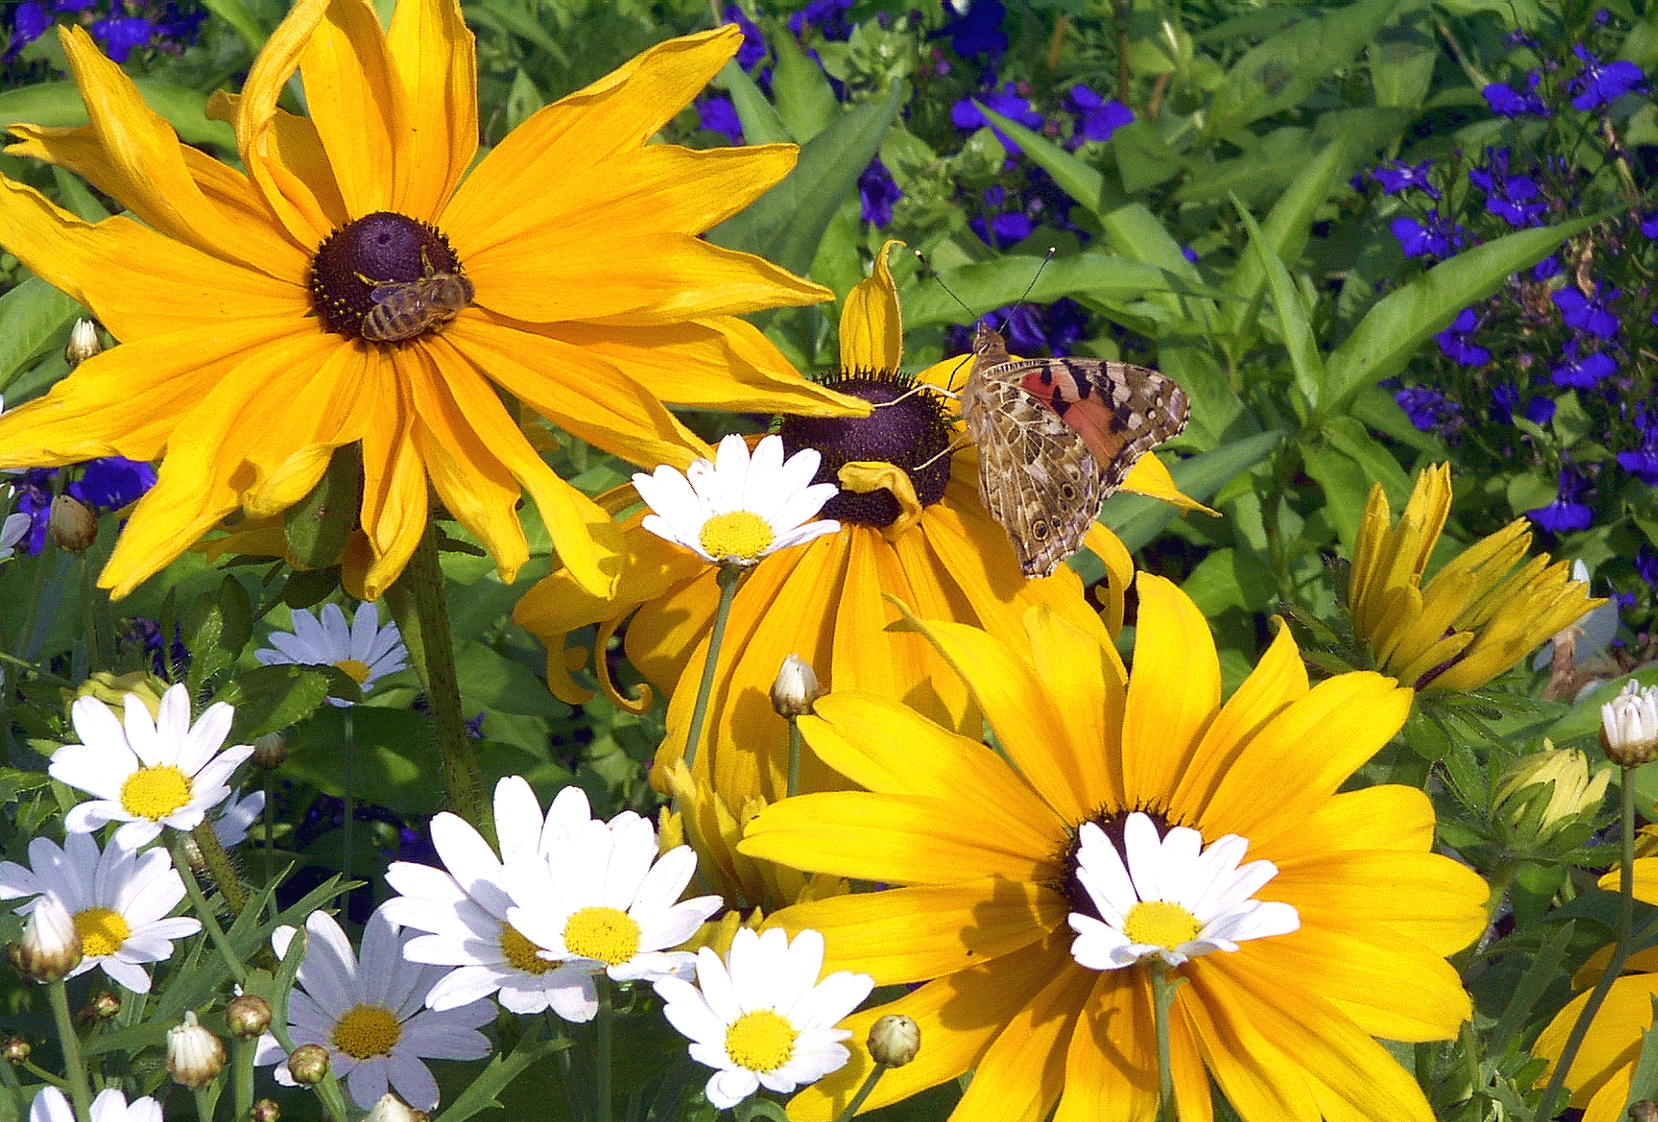
\includegraphics[scale=0.2]{figs/Blume.jpeg}
	\caption{dies ist eine schöne Blume}
	\label{fig:Blume} 
\end{figure}
\noindent
\cref{eq:Formel} zeigt ein Beispiel für eine Formel.
\begin{align}\label{eq:Formel}
	I = \int_{t_0}^{t_0+n \cdot h} f(t) \hspace{0.1cm} dt
\end{align}
\noindent
\cref{tab:Tabelle} zeig ein Beispiel für eine Tabelle
\begin{table}[H]
	\flushleft
	\caption{Tabelle}
	\label{tab:Tabelle} 
	\vspace{0.2cm}
	\begin{tabularx}{\textwidth}{p{3.5cm}XXXXXXX}
		\toprule[1.5pt]
		ABC: & 1 & 2 & 3 \\
		\midrule[1.0pt]
		DEF: & 4 & 5 & 6 \\
		\bottomrule[1.5pt]	
	\end{tabularx}
\end{table}
\noindent
Zitiert wird mit "footcite". Das sieht dann so \footcite[Vgl.][S. 456]{ABC2017} oder so\footcite[Vgl.][S. 123]{DEF2014} aus.
%
\subsection{Unterkapitel 1}\label{subsec:Unterkapitel1}
%
%
\subsection{Unterkapitel 2}\label{subsec:Unterkapitel2}
%
\subsubsection{Unterkapitel 2.1}\label{subsec:Unterkapitel2.1}
%
%
%


